\documentclass{beamer}
% October 2017 
% Author: Dr. Rachid Hourizi and Dr. Michael Wright 
% Department of Computer Science, University of Bath
\usepackage{listings}
\usetheme{Boadilla} 
\lstset{language=C}

\begin{document}

\AtBeginSection[]{
  \begin{frame}
  \vfill
  \centering
  \begin{beamercolorbox}[sep=8pt,center,shadow=true,rounded=true]{title}
    \usebeamerfont{title}\insertsectionhead\par%
  \end{beamercolorbox}
  \vfill
  \end{frame}
}

\title{CM 10227/50258: Lecture 1}
\author{Dr. Rachid Hourizi and Dr. Michael Wright }
\date{\today}
\frame{\titlepage}
\frame{ 

\frametitle{Table of Contents}
\tableofcontents{}}

\section{Introduction}
\begin{frame}
Aims

\begin{itemize}
\item This course provides an introduction to programming

\begin{itemize}
\item problem analysis
\item requirements elicitation
\item design
\item code writing
\item evaluation
\item problem identification and repair (debugging)
\item maintenance
\item extension
\end{itemize}
\end{itemize}
\end{frame}

\begin{frame}
Outcomes

\begin{itemize}
\item On completion of the course, you will be able to

\begin{itemize}
\item Design, implement, test and evaluate programs using

\begin{itemize}
\item a procedural paradigm (using a small subset of the C programming language)
\item an object oriented paradigm (using the Java programming language)
\end{itemize}
\item Understand and use key data structures
\end{itemize}
\end{itemize}
\end{frame} 

 \begin{frame}

Labs, Lectures and Other Sessions

\begin{itemize}
\item In order to help you to learn the concepts at the heart of the course, we provide the following sessions each
week:

\begin{itemize}
\item 2 hour lecture
\item 1 hour tutorial
\item Lab sessions

\end{itemize}
\end{itemize}
\end{frame} 

\begin{frame}

If you need additional help, we also provide

\begin{itemize}
\item \begin{itemize}
\item 15 minute drop in sessions: Sign up in advance from week 4
\item Peer assisted learning sessions: No sign up needed
\end{itemize}
\item Each of these sessions should be on your timetables
\item Details can also be found on Moodle
\end{itemize}
\end{frame} \begin{frame}

\begin{itemize}
\item If, on the other hand, you find the first few lab exercises easy, we would like to give you the opportunity to
stretch yourselves!
\item With that in mind, we will also be running advanced programming labs from weeks 4-11
\item Those labs are

\begin{itemize}
\item mainly aimed at those with stronger programming experience
\item Focused on ``competitive programming'' i.e. programming competitions such as UPIEPC and NWERC

\end{itemize}
\item We will circulate details of the Advanced programming exercise once the main labs are underway
\end{itemize}
\end{frame} 

\begin{frame}

Assessment (CM10227)

\begin{itemize}
\item The course is assessed in two parts

\begin{itemize}
\item 50 percent exam

\begin{itemize}
\item 1 exam in January 2018
\end{itemize}
\item 50 percent coursework

\begin{itemize}
\item 6 smaller lab sheets (or an equivalent 'advanced programming' exercise)
\item 2 larger courseworks
\end{itemize}
\end{itemize}
\item I will go into more detail about each part of this assessment in the second lecture
\end{itemize}

\bigskip
\textbf{PLEASE NOTE THAT YOU MUST ACHIEVE A PASS - I.E. 40 PERCENT OR ABOVE - IN BOTH COURSEWORK AND EXAM IN ORDER TO PASS THIS COURSE}

\end{frame} 
\begin{frame}

Assessment (CM50258)

\begin{itemize}
\item The course is assessed in two parts

\begin{itemize}
\item 50 percent exam

\begin{itemize}
\item 1 exam in January 2018
\end{itemize}
\item 50 percent coursework

\begin{itemize}
\item 3 smaller lab sheets
\item 1 larger programming coursework
\item 1 code analysis and extension
\end{itemize}
\end{itemize}
\item We will go into more detail about each part of this assessment in your first lab
\end{itemize}

\bigskip
\textbf{PLEASE NOTE THAT YOU MUST ACHIEVE A PASS - I.E. 40 PERCENT OR ABOVE - IN BOTH COURSEWORK AND EXAM IN ORDER TO PASS THIS COURSE}

\end{frame} 

\begin{frame}

Moodle

\begin{itemize}
\item More detail on both learning sessions (lectures, labs etc.), coursework and other information about the course can
be found on our Moodle pages:

\begin{itemize}
\item \url{http://moodle.bath.ac.uk/course/view.php?id=30475}
\item \url{https://moodle.bath.ac.uk/course/view.php?id=57411}
\end{itemize}
\item Please check these Moodle pages regularly
\item They will be used for announcements and distribution of material for lectures, labs, coursework
\item We will put copies of the lecture slides on Moodle each week (after the lectures)
\item Along with other information about the coursework

\begin{itemize}
\item e.g. a more detailed version of the aims and objectives shown on previous slides
\end{itemize}
\end{itemize}
\end{frame} 

\begin{frame}

Support

\begin{itemize}
\item If you have questions, we are more than happy to help
\item But please take the initiative

\begin{itemize}
\item Ask the lecturers
\item Ask the lab tutors
\item Use the Moodle forums

\begin{itemize}
\item Though please don{}'t post code on them
\end{itemize}
\item Use the mailing list \href{mailto:programming1@lists.bath.ac.uk}{programming1@lists.bath.ac.uk}
\item Copies of both your Moodle forum posts and your mailing list questions will be sent to the lecturers and all the
tutors
\end{itemize}
\item Contacting us as a group is (very) likely to get a faster response than contacting any one person individually
\end{itemize}
\end{frame}

\begin{frame}
Additional resources
\begin{itemize}
\item You should get into the habit of supplementing course material with your own reading e.g.
\begin{itemize}
\item Kelley and Pohl, 2003, ``C by dissection'' 
\item McDowell and Pohl, 2006, ``Java by dissection''
\end{itemize}
\item remember that you can buy books second hand (e.g. from abebooks.co.uk) as well as new (e.g. from amazon.co.uk)
\end{itemize}
\end{frame} 

\begin{frame}
Additional resources
\begin{itemize}
\item You should also use the internet as a source of information e.g.
\begin{itemize}
\item Google
\begin{itemize}
\item the name of a concept that you dont understand (e.g. ``recursion'')
\item an instruction that isnt working as you expected
\item undesired compiler output
\item etc.
\end{itemize}
\item Get familiar with the places that professional programmers give/offer advice e.g. 
\begin{itemize}
\item stackoverflow.com
\end{itemize}
\end{itemize}
\end{itemize}
\end{frame} 

\begin{frame}
Other support
\begin{itemize}
\item Whilst you should be targeting professional programmers' discussions with your reading, you may, occasionally find that you need to review the fundamentals of a programming topic.
\item In that case, consider the possibility of an onlne tutorial (from KhanAccademy, Udemy etc.).
\item As a starting point, you may want to consider the list of providers here:
\begin{itemize}
\item https://www.upwork.com/blog/2014/02/10-top-sites-online-education/
\end{itemize}
\item Be aware, however, that we will examine and assess your progress against our curriculum rather than theirs. Make sure that you are familiar with all the material on our slides 
\item \textbf{Please tell us if you are struggling. As a rule of thumb, if you feel that you need the ``from scratch'' support provided by an online tutorial, you should also be asking for help from the lab tutors and/or Michael/Rachid}
\end{itemize}
\end{frame}

\begin{frame}
Other support
\begin{itemize}
\item Other forms of support include 
\begin{itemize}
\item Your personal tutor
\item The computer society
\item Peers (as long as you do not work together for classwork)
\end{itemize}
\end{itemize}
\end{frame} \begin{frame}

Plagiarism

\begin{itemize}
\item Do, however, be careful of plagiarism and collusion

\begin{itemize}
\item Reuse: Acknowledging someone else's work (fine)
\item Plagiarism: Presenting someone else's work as your own (bad)
\item Collusion: Working closely with others when work is meant to be individual (bad)
\end{itemize}
\end{itemize}
\end{frame} \begin{frame}

How to succeed on this course

\begin{itemize}
\item Attend the lectures
\item Attend the labs
\item Spend time on this unit outside the lectures and labs
\item \textbf{Do not wait until the last minute to do your work}
\item Get programming experience
\item Don't be afraid to make mistakes; learn from them
\end{itemize}
\end{frame} \begin{frame}

How to succeed on this course: time

\begin{itemize}
\item This course represents 2/5 of your credits this semester
\item Assuming 37.5 working hours per week
\item Then you can assume (as we do) that this course will take 15 hours per week
\item Assuming 3 hours in lectures and tutorials
\item And a minimum of two hours in labs
\item This leaves 10 hours for you to 

\begin{itemize}
\item do further research into your programming
\item and practise what you learn
\end{itemize}
\item Please use them!
\end{itemize}
\end{frame}

\section{First Programs}
\begin{frame}
\frametitle{What is a program and what is programming?}
\begin{itemize}
\item A program is a set of instructions that tells a computer how to perform a computation
\item Example computations include
item Mathematical computations
\begin{itemize}
\item solving a system of equations
\item finding the roots of a polynomial
\end{itemize}
\item Symbolic computations
\begin{itemize}
\item Searching and replacing text in a document
\item Interpreting text in a file (e.g. interpreting another program)
\end{itemize}
\end{itemize}
\end{frame}

\begin{frame}
\begin{itemize}
\item {
Programming can be thought of as the process of breaking a large, complex real world task up into smaller and smaller
sub-tasks until eventually the sub-tasks are simple enough to be performed with a simple (programmable) instruction. e.g.}
\begin{itemize}
\item
Get data from the keyboard, or a file, or some other device.
\item Perform basic mathematical operations e.g. addition and/or multiplication. 
\item Check for certain conditions and execute an appropriate sequence of statements in line with those condition 
\item Perform some action repeatedly, usually with some variation 
\item Display data on the screen or send data to a file or other device. 
\end{itemize}
\end{itemize}
\end{frame}

\begin{frame}
\begin{itemize}
\item It is helpful think of two types of programming languages: 
\begin{itemize}
\item High-level 
\begin{itemize}
\item Java 
\item Python 
\item C++ 
\item Perl 
\item C (arguably)
\end{itemize}
\item Low-level (assembly or machine languages) - Computer specific 
\begin{itemize}
\item Intel x86 (Pentium), Apple - IBM PC compatibles 
\item Motorola/ IBM PowerPC - IBM workstations and servers 
\item Sun SPARC - Sun workstations and servers 
\end{itemize}
\end{itemize}
\item Computers only execute low level languages. 
\item Programs written in high level languages are {}'translated{}' to the machine language of the specific computer. 
\end{itemize}
\end{frame}

\begin{frame}
\begin{itemize}
\item Advantages of low-level programming languages:

\begin{itemize}
\item program can be tuned to specific computer for maximum execution speed and minimum memory consumption. 
\end{itemize}
\item Advantages of high-level programming languages: 

\begin{itemize}
\item Easier to program 
\item Less time to write 
\item Easier for people to read 
\item Easier for people to correct
\item Much easier to port, or modify to run on different computers 
\end{itemize}
\item Today almost all programs are written in high-level programming languages. 
\end{itemize}
\end{frame}

\begin{frame}

A specific programming language: C

\begin{itemize}
\item In the first part of this course, we will use the C programming language as a basis for discussing the
specification, testing, repair and documenting introduced in previous slides
\item (In the second part we will use Java as a basis for further discussion)
\end{itemize}

\end{frame} 

\begin{frame}[fragile]

A first C program: HelloWorld.c

\begin{block}{}
\begin{lstlisting}
/* Hello World program */
#include <stdio.h>

main()
{
	printf("Hello World");
}
\end{lstlisting}
\end{block}

\begin{block}{}
\begin{lstlisting}
Hello World
\end{lstlisting}
\end{block}

\end{frame}


\begin{frame}
\begin{itemize}
\item The code on the previous slide prints the phrase ``Hello World'' on whichever \ device you are using to receive
output (usually a screen).
\item You will notice that it takes quite a lot of code simply to produce that output
\item It is worth taking a moment to discuss each part of that code
\end{itemize}
 
\end{frame}

\begin{frame}[fragile]
\begin{itemize}
\item The first part of the code is a simply a note to the programer(s) 
\end{itemize}
\begin{block}{}
\begin{lstlisting}
/* Hello World program */
\end{lstlisting}
\end{block}
\begin{itemize}
\item In this case, the text is marked as a comment by /* at the start of the line and */ at the end
\end{itemize}

\end{frame} 



\begin{frame}
\begin{itemize}
\item Commenting is an absolute must.
\item It allows you to

\begin{itemize}
\item explain your code
\item refresh your memory when you return to it
\item help others to read your code
\item re-use your code
\end{itemize}
\item We will be giving marks for comments in your coursework (and taking them off when you dont provide them)
\end{itemize}

 

\end{frame} 

\begin{frame}[fragile]
 
\begin{itemize}
\item The two following approaches can both be used to insert comments into C code
\end{itemize}
 
\begin{block}{}
\begin{lstlisting}
/* Everything ignored on one line */ 

and

/* Everything ignored on
* each
* line of text
* marked as part
* of a continuous comment
*/
\end{lstlisting}
\end{block}

\end{frame}


\begin{frame}[fragile]
\begin{itemize}
\item The second line of code tells the compiler to use (``include'') code from another file 
\end{itemize}

\begin{block}{}
\begin{lstlisting}
#include <stdio.h>
\end{lstlisting}
\end{block}

\begin{itemize}
\item This allows us to re-use code that has already been written -- another important concept to which we will return later
\end{itemize}

\end{frame} 

\begin{frame}[fragile]

\begin{itemize}
\item The third line of code tells the compiler that the following lines i.e. everything between \{ and \} makes up the main part of the program
\item When the program is run, the first of those lines will be executed first
\item The name given to the code marked as main() is ``The main() function''
\item Every C program must have a main() function
\end{itemize}

\begin{block}{}
\begin{lstlisting}
main()
{
	code goes here
}\end{lstlisting}
\end{block}


\end{frame} 

\begin{frame}[fragile]

\begin{itemize}
\item The next line of code (i.e. the content of the main() function)is the part \ that does the printing:
\end{itemize}

\begin{block}{}
\begin{lstlisting}
printf("Hello World");
\end{lstlisting}
\end{block}
\end{frame} 

\begin{frame}[fragile]
\begin{itemize}
\item It is useful to think of this code in two parts -- the command or function that tells the
computer what to do:
\end{itemize}

\begin{block}{}
\begin{lstlisting}
printf();
\end{lstlisting}
\end{block}

\begin{itemize}
\item and the (input) data to which that command is applied
\end{itemize}

\begin{block}{}
\begin{lstlisting}
"Hello World"
\end{lstlisting}
\end{block}

\begin{itemize}
\item it is also worth noting that the line ends with a semicolon (``;'')
\item C uses a semicolon to indicate the end of each instruction 
\end{itemize}
\end{frame}

\begin{frame}
\begin{itemize}
\item Before looking at the ``Hello World'' example
\item We introduced the idea of instructions written in ``High-level'' programming languages being ``translated'' to machine specific instructions
\end{itemize}
\end{frame}

\begin{frame}
\begin{itemize}
\item The translation of programs written in high level languages to machine specific instructions can be achieved in more than one way:
\item We can for example use an Interpreter

\begin{itemize}
\item Input (Code) $\rightarrow $ \ Interpreter $\rightarrow $ Final Output

\begin{itemize}
\item The Interpreter reads in the (high level) source code
\item After interpretation, the final output is delivered to the user e.g. appears on a screen
\end{itemize}
\end{itemize}
\end{itemize}
\end{frame}

\begin{frame}

\begin{itemize}
\item An alternative approach is to use a compiler

\begin{itemize}
\item Input code $\rightarrow $ Compiler $\rightarrow $ Object Code $\rightarrow $ Execution $\rightarrow $ Output
\begin{itemize}
\item The compiler reads in the source code
\item and generates object code as output
\item you execute that object code (one way or another)
\item and the end result is delivered to the user e.g. appears on a screen
\end{itemize}
\end{itemize}
\end{itemize}
\end{frame}

\begin{frame}
\begin{itemize}
\item All high level programming languages (e.g. C, Java, Python) can, in theory be interpreted or compiled.
\item As we will see when we move to Java later in the course, more complex conversions also exist 
\begin{itemize}
\item e.g. compilation to an intermediate form of code which is then interpreted
\end{itemize}
\item Usually, however, a 'standard' set of tools are provided that follow one route or another 
\item In that context, you will hear discussion of C, Python and Java being 'Compiled languages' (since the standard tools provided follow the compilation route)
\item We will use that convention in this course
\end{itemize}
\end{frame}

\begin{frame}
In order to compile and run our example \ C program ``Hello World'' on a University UNIX or Windows machine:
\begin{itemize}
\item create a file called HelloWorld.c
\item Note: use a plain text editor such as Notepad++ or emacs (Do not use Word)
\item save it in a location that you can find again from the command line
\item navigate to that location and run the gnu compiler:
\end{itemize}
continued on next slide
\end{frame}


\begin{frame}
\begin{itemize}
\item Then type the following command
\begin{itemize}
\item gcc HelloWorld.c  
\item Note: You can use other variations of this command - see below. 
\item To start with, however, stick to this one
\end{itemize}

\item When the compiler has compiled (and linked) your program it will create an executable (runnable) version. By
default, that executable version of your program will be called a.out on a UNIX machine and a.exe on a Windows machine
\item you can now run the executable version of your program by typing ./a.out on the command line 
\item You should now see the output generated by the program 
\end{itemize}
\end{frame}

\begin{frame}
\begin{itemize}
\item \textbf{We have put a video on moodle showing the compilation and execution of a program being compiled and run}
\item the tutors will help you with compilation and running a program locally in the first lab
\item either way, it is a useful exercise to copy the HelloWorld program at the start of this section and make sure that you can compile and run it without making any changes
\end{itemize}
\end{frame}


\begin{frame}
\begin{itemize}
\item If you have never compiled and run a program before, you can try entering your code into the online environment at https://www.codechef.com/ide
\item that environment handles the compilation and run steps for you
\item It allows you to enter your code and (after pressing a button) see the results of running your code on screen
\item Make sure however that you have chosen C (Gcc-4.9.2) in the box above the coding area
\end{itemize}
\end{frame}


\begin{frame}[fragile]

\begin{itemize}
\item In the HelloWorld example, above, the text (more formally a ``String'' of characters) can of course be replaced
with different text (a different ``String'').
\item We could, for example, print ``Goodbye World'':
\end{itemize}

\begin{block}{}
\begin{lstlisting}
/* Goodbye World program */
#include <stdio.h>

main()
{
	printf("Goodbye World");
}
\end{lstlisting}
\end{block}

\begin{block}{}
\begin{lstlisting}
Goodbye World
\end{lstlisting}
\end{block}

\end{frame}

\begin{frame}[fragile]
 
\begin{itemize}
\item We could also use two printf() commands to print both Strings to the screen:
\end{itemize}

 \begin{block}{}
\begin{lstlisting}
/* Hello World program */
#include <stdio.h>
main()
{
	printf("Hello World \n");
	printf("Goodbye World");
}
\end{lstlisting}
\end{block}

\begin{block}{}
\begin{lstlisting}
Hello World
Goodbye World
\end{lstlisting}
\end{block}

\begin{itemize}
\item Note the use of the newline (\textbackslash n) at the end of the first print statement. Without that newline, the program would try to print both statements on the same line
\end{itemize}

\end{frame}

\begin{frame}[fragile]

\begin{itemize}
\item We would, however, have to recompile and re-run the code once we had made that change in order to see the new
String printed to the screen
\item Strings which cannot be changed once the program is running (e.g. ``Hello World'' and ``Goodbye World'', above)
are described as String ``literals''.
\end{itemize}
\end{frame}

\begin{frame}
\begin{itemize}
\item A more flexible approach to printing data to the screen is to use a variable whose value can be changed whilst the program is running ("at runtime")
\end{itemize}
\end{frame} 

\begin{frame}[fragile]
Variables
\begin{itemize}
\item Variables can be thought of as named containers (locations in memory) that hold some information (a value)
\end{itemize}
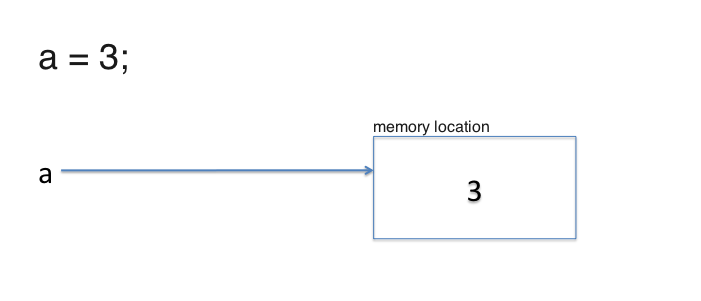
\includegraphics[scale=0.5]{Slide2.png}
\end{frame}

\begin{frame}[fragile]
Variables
\begin{itemize}
\item In C all variables have a 'type' -- i.e. a description of the data that can be held within the named container
\item Providing a description of the `type' allows the C compiler to allocate an appropriate amount of memory for data held within the container.
\end{itemize}
\end{frame}

\begin{frame}[fragile]
Variables
\begin{itemize}
\item When discussing variables (and many other programming topics), you will find that a shorthand descripton is often used to describe that variable (named location in memory that holds a value)
\begin{itemize}
\item There is sufficient memory reserved at the location assiciated with the name `a' to hold an integer becomes
\item the variable `a' refers to an integer or
\item a is an integer
\end{itemize}
\end{itemize}
\end{frame}


\begin{frame}[fragile]
Variables
\begin{itemize}
\item A full list of C variable (or data) types can be found online
\item but at this point, you dont need to understand them all
\item to start with, we will focus on just three:
\begin{itemize}
\item variables that refer to an integer are of type int
\item variables that refer to a floating point number are of type float
\item variables that refer to a floating point number that is allocated (approximately) double the amount of memory allocated to a float are of type double
\end{itemize}
\end{itemize}
\end{frame}

\begin{frame}[fragile]
\begin{block}{}
\begin{lstlisting}
/*declaration and assignment 
*of an integer (int) variable named myInt
*and a float named myFloat
*/
int myInt=7;
float myFloat=7.264;
\end{lstlisting}
\end{block}
\end{frame}

\begin{frame}
\begin{itemize}
\item You \textbf{declare} a variable by specifying its type and name
\begin{itemize}
\item int myInt
\end{itemize}
\item \textcolor{black}{You }\textbf{\textcolor{black}{instantiate }}\textcolor{black}{ a variable the first time that you assign a value to it}
\begin{itemize}
\item {\color{black} myInt=7;}
\end{itemize}
\item You can continue to assign values to a variable (overwriting the previous value each time)
\begin{itemize}
\item myInt\textcolor{black}{=24;}
\end{itemize}
\end {itemize}
\end{frame}

\begin{frame}
\begin{itemize}
\item If you try to access a name before it is been properly created (declared and instantiated), you will get an error or the program will crash.
\end{itemize}
\end{frame}

\begin{frame}[fragile]
\begin{itemize}
\item This code prints the integer 7 to the screen
\end{itemize}
\begin{block}{}
\begin{lstlisting}
/* Print an Integer */
#include <stdio.h>
main()
{
  int a=7;
  printf("The integer is %d\n", a);
}
\end{lstlisting}
\end{block}

\begin{block}{}
\begin{lstlisting}
The integer is 7
\end{lstlisting}
\end{block}

\end{frame}

\begin{frame}[fragile]
\begin{itemize}
\item This code does not print a to the screen (it returns an error or crashes the program)
\end{itemize}
\begin{block}{}
\begin{lstlisting}
/* Print an Integer */
#include <stdio.h>
main()
{
 printf("Integer that you have entered is %d\n", a);
 int a=7;
}
\end{lstlisting}
\end{block}

\end{frame}


\begin{frame}[fragile]
\begin{itemize}
\item Note that the \%d in the printf() statement in these examples
\item \%d is an example of a format specifier
\item It tells printf() that an integer should be included as part of the string to be printed (or more specifically, a decimal integer, hence the 'd')
\item The integer (i.e. the one refered to by a) is then specified after a comma
\item you will need to use a format specifier each time you try to include a variable in your print statements
\end{itemize}

\end{frame}

\begin{frame}[fragile]
\begin{itemize}
\item The format specifier for a floating point number (i.e. a float or a double) is \%f
\end{itemize}
\begin{block}{}
\begin{lstlisting}
#include <stdio.h>
main()
{
 float a=32.654;
 printf("the float held in a is %f\n", a);
 a=1.7;
 printf("the float held in a is %f\n", a);
 a=156.797;
 printf("the float held in a is %f\n", a);
}
\end{lstlisting}
\end{block}

\begin{block}{}
\begin{lstlisting}
the float held in a is 32.653999
the float held in a is 1.700000
the float held in a is 156.796997
\end{lstlisting}
\end{block}

\end{frame}

\begin{frame}
\begin{itemize}
\item C is pretty liberal in the range of names that it allows you to use for variables:
\item Characters which may be used in a C variable name include
\begin{itemize}
\item Underscore (\_)
\item Upper Case Letters (A-Z)
\item Lower Case Letters (a-z)
\item Digits (0-9)
\end{itemize}
\item so permissable variable names include a, \_myInt and \_myInt99
\end{itemize}
\end{frame}

\begin{frame}
\begin{itemize}
\item Some characters may not, however, be used in variable names:
\item Blanks and commas may not be used
\item special symbols other than underscore may not be used

\item first character should be an upper case character, a lower case character or an underscore
\end{itemize}
\end{frame}


\begin{frame}
\begin{itemize}
\item there are also some reserved words (words that C reserves for specific uses), which may not be used
\item you cannot, for example use the word int as a variable name since C reserves it for use as a type identifier (see previous slides)
\item a list of reserved words can be found at http://crasseux.com/books/ctutorial/Reserved-words-in-C.html
\end{itemize}
\end{frame}

\begin{frame}
Building more complex computations: Some vocabulary
\begin{itemize}
\item an \textbf{operator} is a character which describes an action to be carried out
\item the actions themselves are called operations
\begin{itemize}
\item +, -, *, / and = are all operators
\bigskip
\end{itemize}
\item \textcolor[rgb]{0.13333334,0.13333334,0.13333334}{a
}\textbf{\textcolor[rgb]{0.13333334,0.13333334,0.13333334}{statement
}}\textcolor[rgb]{0.13333334,0.13333334,0.13333334}{is the smallest standalone element of a
}\textbf{\textcolor[rgb]{0.13333334,0.13333334,0.13333334}{programming
}}\textcolor[rgb]{0.13333334,0.13333334,0.13333334}{language which expresses some action to be carried out
}\textcolor[rgb]{0.13333334,0.13333334,0.13333334}{}
\begin{itemize}
\item \textcolor[rgb]{0.13333334,0.13333334,0.13333334}{e.g. }\textcolor[rgb]{0.13333334,0.13333334,0.13333334}{an
assignment statement:}
\begin{itemize}
\item {\color[rgb]{0.13333334,0.13333334,0.13333334}
int a = 5;}
\end{itemize}
\end{itemize}
\item \textbf{statements} can contain any number of operations 
\begin{itemize}
\item e.g. int a=1+2*3/4-5+6-7*8/9
\end{itemize}
\bigskip
\item \textbf{An expression} is a combination of constants, variables, operators and functions that .. produces another value
\begin{itemize}
\item e.g. 1+2*3/4-5+6-7*8/9 in the statement above.
\end{itemize}
\end{itemize}
\end{frame}

\begin{frame}[fragile]
\begin{itemize}
\item We can use printf() to print the value of an expression
\end{itemize}
\begin{block}{}
\begin{lstlisting}
#include <stdio.h>
main()
{
 int a=4;
 printf("twice the value of a is %d\n", a+a);
 printf("three times the value of a is %d\n", 3*a);
 printf("half four times a is %d\n", 4*a/2);
}
\end{lstlisting}
\end{block}

\begin{block}{}
\begin{lstlisting}
twice the value of a is 8
three times the value of a is 12
half four times a is 8
\end{lstlisting}
\end{block}
\end{frame}

\begin{frame}[fragile]
\begin{itemize}
\item note the use of the mathematical operators +,-, * (multiply) and / (divide)
\end{itemize}


\end{frame}


\begin{frame}
\begin{itemize}
\item When more than one operator appears in an expression the order of evaluation depends on the
\textcolor[rgb]{0.26666668,0.0,0.5176471}{rules of precedence}. 
\item C follows the same rules as mathematics: PMDAS 

\item Parenthesis have highest precedence

\begin{itemize}
\item used to force desired evaluation order: 
\begin{itemize}
\item 2*(3-1) is 4, and (1 + 1)*(5-2) is 6
\end{itemize}
\item can also be used to make expression easier to read:
\begin{itemize}
\item (\textit{minute * }100)\textit{/}60 
\end{itemize}
\end{itemize}
\item Multiplication and Division have the same precedence, which is higher than Addition and Subtraction, which also have the same precedence. 
\begin{itemize}
\item 2*3-1 yields 5 rather then 4, and 2\textit{/}3-1 is -1, not 1 
\end{itemize}
\end{itemize}
\end{frame}

\begin{frame}
\begin{itemize}
\item NB dividing one integer by another (e.g. 22/7) returns another integer (3) rather than a more accurate result (3.1428)

\item If you want to return a floating point result, you need to use at least one floating point value in the original

\begin{itemize}
\item 22.0/7
\item 22/7.0
\item 22.0/7.0 
\end{itemize}
\end{itemize}
\end{frame}

\begin{frame}
\begin{itemize}
\item mathematical functions

\begin{itemize}
\item There are, of course, situations in which we might want to perform more complex computations than can easily be achieved simply through addition, subtraction, division and multiplication
\item We might, for example want to be able to calculate the sqare root of a number or raise a second number to a power 
\end{itemize}
\end{itemize}
\end{frame}

\begin{frame}
\begin{itemize}
\item One approach to performing these computations is to write code to do within each program requiring that functionality
\item A much simpler route to achieving the same goal, however, is to see whether someone else has written the code that you need and use theirs
\item Whether you write that code yourself or use some that has been written by other people, it is likely that you will want to collect together operations, expressions and or statements into \textbf{functions} that perform the necessary computations for you
\end{itemize}
\end{frame}

\begin{frame}
\begin{itemize}
\item \textbf{functions} are procedures or routines which do something with the data given to them (e.g. printf(), main()).
\item note that some programming languages make a distinction between a \textbf{function}, which returns a value, and a \textbf{procedure}, which performs some operation but does not return a value
\item we will return to the definition of \textbf{functions} shortly
\end{itemize}
\end{frame}

\begin{frame}
\begin{itemize}
\item for many common mathematical computations, pre-written code is provided in files that are installed as standard with the C programming language
\item those files are collectively known as the C libraries
\end{itemize}
\end{frame}

\begin{frame}
\begin{itemize}
\item Pre-defined mathematical functions continued
\begin{itemize}
\item More specifically, common mathematical functionality is provided through a set of 'functions' that are contained in the math library
\item A function is a named sequence of statements that performs a desired operation (such as calculate a square root or raise a number to a power) 
\item We have already seen a C library function being used in the HelloWorld program
\item i.e. the printf() function is provided by a library accessed via stdio.h 
\item (actually, we have seen two functions, the second is the main() function, which *is not* pre-defined in a C library - we have been writing that one ourselves)
\end{itemize}
\end{itemize}
\end{frame}

\begin{frame}[fragile]
\begin{itemize}
\item Before we can use C's pre-defined mathematical functions, we need to tell the compiler how to find them
\begin{itemize}
\item e.g. a function which, when provided with a number as input, gives us the square root of that number as output
\item e.g. a function which, when provided with two numbers as input, gives us the first number raised to the power of the second number as output
\end{itemize}
\item i.e. we need to tell the compiler that the location of these functions is provided in a file called math.h 
\end{itemize}
\end{frame}

\begin{frame}[fragile]
\begin{itemize}
\item If we want to use those functions, we must explictly include math.h in our code
\end{itemize}
\begin{block}{}
\begin{lstlisting}
/* Print three floating point numbers */
#include <stdio.h>
#include <math.h>
main()
{
 do something;
 printf(the result of doing something);
}
\end{lstlisting}
\end{block}
\end{frame}

\begin{frame}[fragile]
\begin{itemize}
\item NOTE: When including math.h, you must also add -lm to your compile command
\item i.e. when compiling your code, per the Interpreting, Compiling and Running section, above, 
\item use gcc ProgramName.c -lm 
\item (rather than simply gcc ProgramName.c) 
\end{itemize}
\end{frame}

\begin{frame}
\begin{itemize} 
\item In order to use the printf() function, we used stdio.h to import it
\item We then used the name of that function to ask for a computation to be carried out - printf()
\item And provided input data for that command to be carried out on - "Hello World"
\end{itemize}
\end{frame}

\begin{frame}
\begin{itemize} 
\item in order to calculate the square root of a number, we need to follow a parallel path:
\item include the file describing the location of the function that will be executed
\item use the name of the function in question, which turns out to be sqrt()
\item and provide data of an appropriate type as input to that command - in this case, a double e.g. 4.0
\end{itemize}
\end{frame}

\begin{frame}
\begin{itemize} 
\item in this case, we also need to take an extra step - work out what to do with the result of the calculation
\item the sqrt() function returns us a double 
\item we can store that double in a variable, print it to screen or both
\end{itemize}
\end{frame}

\begin{frame}[fragile]
\begin{block}{}
\begin {lstlisting}
/* program to calculate the square root of x*/
#include <math.h>    
#include <stdio.h>    

int main()    
{    
   
double x = 4.0; 
 
double result = sqrt(x);    
printf("The square root of %f is %f\n", x, result);      
} 
\end{lstlisting}
\end{block}
\begin{block}{}
\begin{lstlisting}
The square root of 4.000000 is 2.000000
\end{lstlisting}
\end{block}
\begin{itemize} 
\item note the inclusion of two variables in the printf() statement
\end{itemize}
\end{frame}

\begin{frame}[fragile]
\begin{block}{}
\begin {lstlisting}
/* program to calculate the yth power of x*/
#include <math.h>    
#include <stdio.h>    

int main()    
{    
double x = 4.0; 
double y = 2.0;
 
double result = pow(x,y);    
printf(" %f to the power of %f is %f", x, y, result);      
}  
\end{lstlisting}
\end{block}

\begin{block}{}
\begin{lstlisting}
 4.000000 to the power of 2.000000 is 16.000000
\end{lstlisting}
\end{block}

\begin{itemize} 
\item note the inclusion of three variables in the printf() statement
\end{itemize}
\end{frame}

\begin{frame}[fragile]
\begin{block}{}
\begin{lstlisting}
The C library function 
double sqrt(double x) 
returns the square root of x

The C library function 
double pow(double x, double y) 
returns x raised to the power of y
\end{lstlisting}
\end{block}
General form:
\begin{block}{}
\begin{lstlisting}
The C library function 
returnedType functionName(input data and types)
returns the result 
	of performing specified computation 
	on the input data
\end{lstlisting}
\end{block}

\end{frame}

\begin{frame}
\begin{itemize}
\item Just like mathematical operators, C functions can be combined within complex expressions

\begin{itemize}
\item 1+sqrt(4);
\item 1+pow(3,2);
\end{itemize}

\item And included directly in print statements

\begin{itemize}
\item printf(" The square root of 4 is \%f ", sqrt(4));
\item printf(" The square root of x is \%f ", sqrt(result));
\end{itemize}

\end{itemize}
\end{frame}

\begin{frame}[fragile]
\begin{itemize}

\item Note also that math.h provides values for some common mathematical constants including pi and e
\item Once you have \#included math.h in your C program, you can refer to those mathematical constants using M\_PI and M\_E
\end{itemize}

\begin{block}{}
\begin{lstlisting}
#include <stdio.h>
#include <math.h>
main()
{
 double x=M_PI;
 double y=M_E; 
 printf("PI plus one equals %f, e= %f", x+1, y); 
}
\end{lstlisting}
\end{block}

\begin{block}{}
\begin{lstlisting}
PI plus one equals 4.141593, e= 2.718282
\end{lstlisting}
\end{block}
\end{frame}

\section{Errors and Debugging}

\begin{frame}
\begin{itemize}
\item As you develop as programers and computer scientists (a key aim of this course), we will encourage you to draw together approaches and techniques that you might expect to find in other disciplines e.g.:  
\begin{itemize}
\item Mathematics 
\begin{itemize}
\item Use formal languages to denote ideas (specifically computations) 
\end{itemize}
\item Engineering
\begin{itemize}
\item Design
\item Assemble components into systems 
\item Evaluate trade-offs among alternatives 
\end{itemize}
\item Natural Science
\begin{itemize}
\item Observe behaviour of complex systems 
\item Form hypotheses
\item Test predictions 
\end{itemize}
\end{itemize}
\end{itemize}	
\end{frame}


\begin{frame}
\begin{itemize}
\item The single most important skill for a computer scientist is \textcolor[rgb]{0.26666668,0.0,0.5176471}{problem solving }
\begin{itemize}
\item Working out how to formulate problems 
\item Thinking creatively about solutions 
\item Expressing solutions clearly and accurately 
\end{itemize}
\item Learning to program is learning to solve problems
\end{itemize}
\end{frame}

\begin{frame}
\begin{itemize}
\item A problem that you will encounter frequently is dealing with programming errors 
\item The results of those errors are more commonly known as called \textcolor[rgb]{0.26666668,0.0,0.5176471}{bugs}. 
\item The process of tracking them down and correcting them is called
\textcolor[rgb]{0.26666668,0.0,0.5176471}{debugging}. 
\item With problem solving, decomposition, \textcolor[rgb]{0.26666668,0.0,0.5176471}{debugging }is one key skills for
successful programers 
\item Bugs are part of the programers life, you cannot escape them, you just have to find them and solve them 
\item Practise makes perfect 
\end{itemize}
\end{frame}

\begin{frame}
\begin{itemize}
\item Syntax Errors
\begin{itemize}
\item The easiest type of error to identify (and, arguably, to make) 
\item C (the language we will be using at the start of this course) cannot execute a program unless it is syntactically correct. 
\item You have the compiler to find them and tell you what is wrong 
\item It returns an error message without starting the program. 
\item Syntax refers to the structure of your program and rules about that structure. 
\end{itemize}
\end{itemize}
\end{frame}

\begin{frame}
\begin{itemize}
\item Example Syntax Errors 
\begin{itemize}
\item In English, a sentence must begin with a capital letter and end with a single full stop. 
\item this sentence contains a syntax error. 
\item So does this one \textcolor[rgb]{0.3372549,0.0,0.64705884}{\ }
\item A C example with mismatched parenthesis: 
\begin{itemize}
\item (5 /2) ) 
\end{itemize}
\end{itemize}
\end{itemize}
\end{frame}

\begin{frame}
\begin{itemize}
\item Run Time Errors
\begin{itemize}
\item Do not occur until the program is run and the particular faulty line is executed. 
\item Called exceptions because something exceptional (and usually bad) has happened. 
\item Execution of your program is normally terminated at this point. 
\item Information about the current state of the program is printed. 
\item Sometimes hard to fix, as they could be input or hardware dependent. 
\item Your code should take this into account. This is called \textcolor[rgb]{0.26666668,0.0,0.5176471}{robustness }
\end{itemize}
\end{itemize}
\end{frame}

\begin{frame}
\begin{itemize}
\item Example Run Time Errors
\begin{itemize}
\item An example when executing a Java program is a division-by-zero error:
\item 5/0 
\end{itemize}
\end{itemize}
\end{frame}

\begin{frame}
\begin{itemize}
\item Logical Errors
\begin{itemize}
\item The program runs successfully: no error messages ... 
\item ... but it does not do what you wanted it to do {\dots}
\item ... instead it does what you told it to do. 
\item Debugging logical errors requires you to work backwards from the observed output (if any) to determine what the program is actually doing internally. 
\end{itemize}
\end{itemize}	
\end{frame}

\begin{frame}
\begin{itemize}
\item Experimental Debugging
\begin{itemize}
\item Debugging is one of the most important skills you will acquire in the unit 
\item Many programers believe debugging is one of the most intellectually rich, challenging, and interesting parts of programming. 
\item Debugging is a form of detective work: 
\begin{itemize}
\item You are confronted with clues, and you have to infer the processes and events that lead to the results you see.
\end{itemize}
\end{itemize}
\begin{itemize}
\item Debugging can also be seen as an experimental science: 
\begin{itemize}
\item Form hypothesis about cause of error. 
\item Modify program, and predict new outcome. 
\item If results match prediction, hypothesis is correct. 
\item Otherwise, modify hypothesis. 
\end{itemize}
\end{itemize}
\end{itemize}
\end{frame}

\begin{frame}
\begin{itemize}
\item {}''\textit{When you have eliminated the impossible, whatever remains, however improbable, must be the truth'' (Sherlock Holmes, from A. Conan Doyle's The Sign of Four) }
\end{itemize}
\end{frame}

\begin{frame}
\begin{itemize}
\item Experimental Programming  and Debugging 
\begin{itemize}
\item At some point, programming and debugging converge: 
\item Programming can be seen as the process of debugging a program until it does what you want. 
\end{itemize}
\end{itemize}
\end{frame}

\begin{frame}
\begin{itemize}
\item Experimental Programming  and Debugging 
\begin{itemize}
\item Start with a working program that does something. 
\item Make small modifications, debugging them as you go. 
\item Always have a working program. 
\item Test-Driven Development and Agile Programming are examples of techniques that use this approach
\item Linux is an example of the output that you can achieve with this kind of approach 
\item Linus Torvalds started out writing a program to explore the Intel 80386 chip. 
\item It simply switched between printing AAAA and BBBB {\dots}. and evolved to Linux! 
\end{itemize}
\end{itemize}
\end{frame}

\begin{frame}
\begin{itemize}
\item While this week's concepts are fresh in your minds (first programs, functions, data, types and errors),
\item We would like you to try a small debugging exercise. 
\item The code on the following slide does not work as intended
\item Work in small groups (approx 3 people) to 
\begin{itemize}
\item identify and fix the errors
\item decide which kind of error has occured in each case (syntax, runtime or logical)
\end{itemize}
\item These lecture notes are now Moodle if you would like to use them
\item And you may use the ide introduced this morning to run the code and get clues about what is going on
\end{itemize}
\end{frame}

\begin{frame}[fragile]

\begin{block}{}
\begin{lstlisting}
/*this code, when run, 
* doesnt give the expected output
* The output should be PI plus c equals 5.141593 
* i.e. the actual result of adding c to PI
* Please find and repair the errors
* So that the program runs as expected
* (It might be useful to categorise the errors)
*/
#include <stdio.h>
main()
{
 int a=7;
 float b= 32.0
 a=62;
 b=17.0;
 printf("PI plus c equals %d", M_PI+b);
 double c=2.0; 
}
\end{lstlisting}
\end{block}
\end{frame}

\section{Next Steps: Coursework and Assessment}
\begin{frame}
\begin{itemize}
\item On Thursday each week, We will put up the coursework exercises that you need complete and hand on the Monday, eleven days later
\item The first set of lab exercises will go up on Thursday October 6th
\item and should be handed in at 5pm on October 17th
\item Each set of exercises is accompanied by a detailed set of instructions
\item The relationship between those exercises and your overall mark for this course is described on the following slides
\end{itemize}
\end{frame}

\begin{frame}
Coursework and Assessment

\begin{itemize}
\item The formal assessment of this course comes from a combination of

\begin{itemize}
\item Coursework (50\%)

\begin{itemize}
\item Lab Exercises
\item Larger Coursework
\end{itemize}
\item A final exam (50\%)
\end{itemize}
\item In order to pass this unit, you will need to obtain a pass mark (40\% or more) in both coursework and exam
\end{itemize}
\end{frame} 

 \begin{frame}

How to succeed: Time management

\begin{itemize}
\item Dont forge that strong time management can make this course feel considerably easier

\begin{itemize}
\item See the Bath Student Union website (url down when we wrote these slides)
\item http://counseling.uchicago.edu/page/asap-time-management 
\end{itemize}
\end{itemize}
\end{frame}

\begin{frame}
Assessment

\begin{itemize}
\item For CM10227, the unit's coursework requirements (50\% of your total marks) can completed in one of two ways:

\begin{itemize}
\item option a):
\begin{itemize}
\item 6 lab exercises
\item plus two larger courseworks
\end{itemize}
\item option b):
\begin{itemize}
\item 2 lab exercises (the first two)
\item plus an advanced programming lab exercise
\item plus two larger courseworks (as above)
\end{itemize}
\end{itemize}
\end{itemize}
\end{frame} 

\begin{frame}
Assessment

\begin{itemize}
\item For CM50258, you have fewer choices:

\begin{itemize}
\item 4 lab exercises
\item one larger coursework
\item plus one code analysis
\end{itemize}
\item Note, however, that you can attempt the other other CM10227 exercises
\item and we will give you indicative marks and feedback for each one
\item though the additional marks will not count towards your grade for the course
\end{itemize}
\end{frame} 

\begin{frame}
Lab Exercises

\begin{itemize}
\item Each of the lab sheets will correspond to one or two lectures
\item Feedback on your solutions can be obtained from the lab tutors
\item You are strongly encouraged to attempt all labs
\end{itemize}
\end{frame} \begin{frame}

Lab Exercises

\begin{itemize}
\item Lab exercises will be marked as follows:
\item Weekly lab sheets

\begin{itemize}
\item 60\%-100\%: 10 marks
\item 40-59\%: 5 marks
\item 0-39\%: 0 marks
\end{itemize}
\item Advanced programming exercise

\begin{itemize}
\item correctly working 25 marks
\item design and program structure: 15 marks
\end{itemize}
\end{itemize}
\end{frame} 

\begin{frame}
Late Submission

\begin{itemize}
\item 1 minute late: 40 percent max
\item 5 days late: 0 percent max
\item Extensions 

\begin{itemize}
\item can only be given by the Director of Studies (Fabio Nemetz)
\item will only be given for special circumstances 
\end{itemize}
\end{itemize}
\end{frame}

\begin{frame}
Marking
\begin{itemize}
\item We use a semi-automated marking tool when grading coursework
\item The tool generates some mark automatically 
\item We then add marks for the quality and style of your code ``by hand''
\item Comments are also written ``by hand''
\end{itemize}
\end{frame}

\begin{frame}
Marking
\begin{itemize}
\item For the first time this year, we have also opened a ``student-facing'' part of that tool
\item Which will allow you to check that your code compiles and run before you submit it
\item (It won't, however, tell you the mark that you will recieve for that code)
\item We will put links to that part of the tool on Moodle with each lab sheet
\item (Note that the tool definitely works in Google Chrome. Performance in other browsers may vary)
\end{itemize}
\end{frame}

\begin{frame}[fragile]
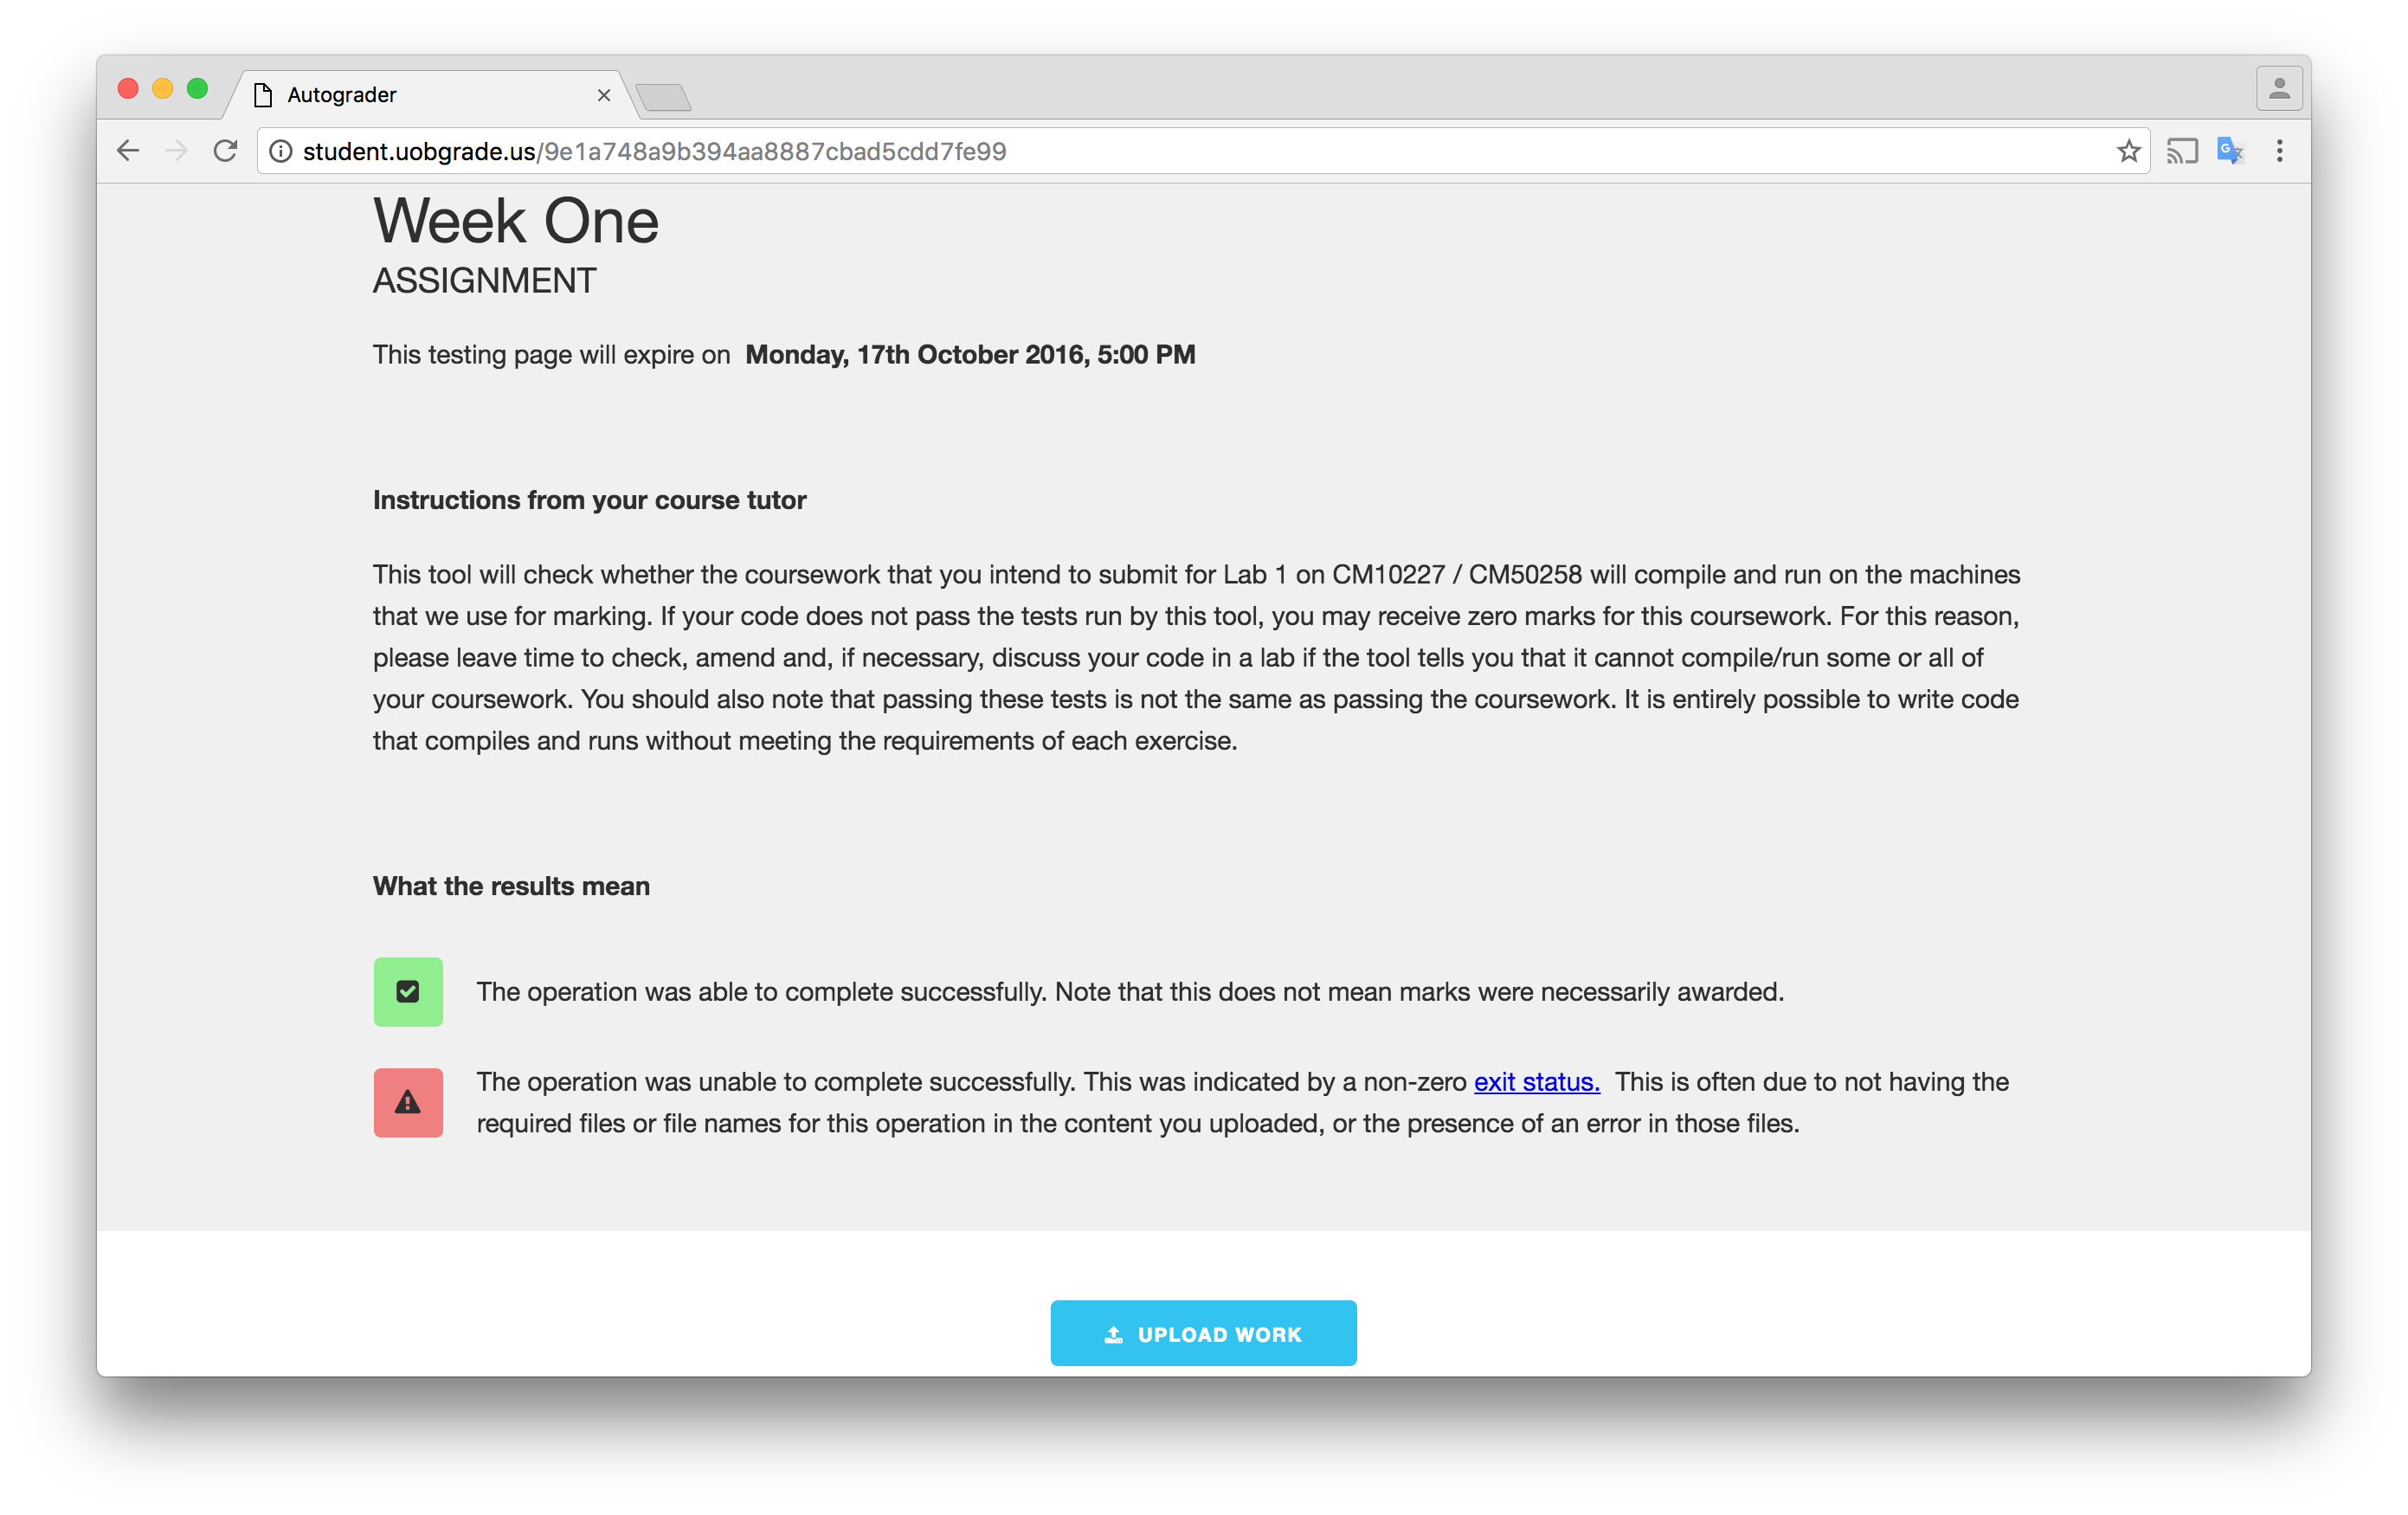
\includegraphics[scale=0.12]{Auto1.png}
\end{frame}

\begin{frame}[fragile]
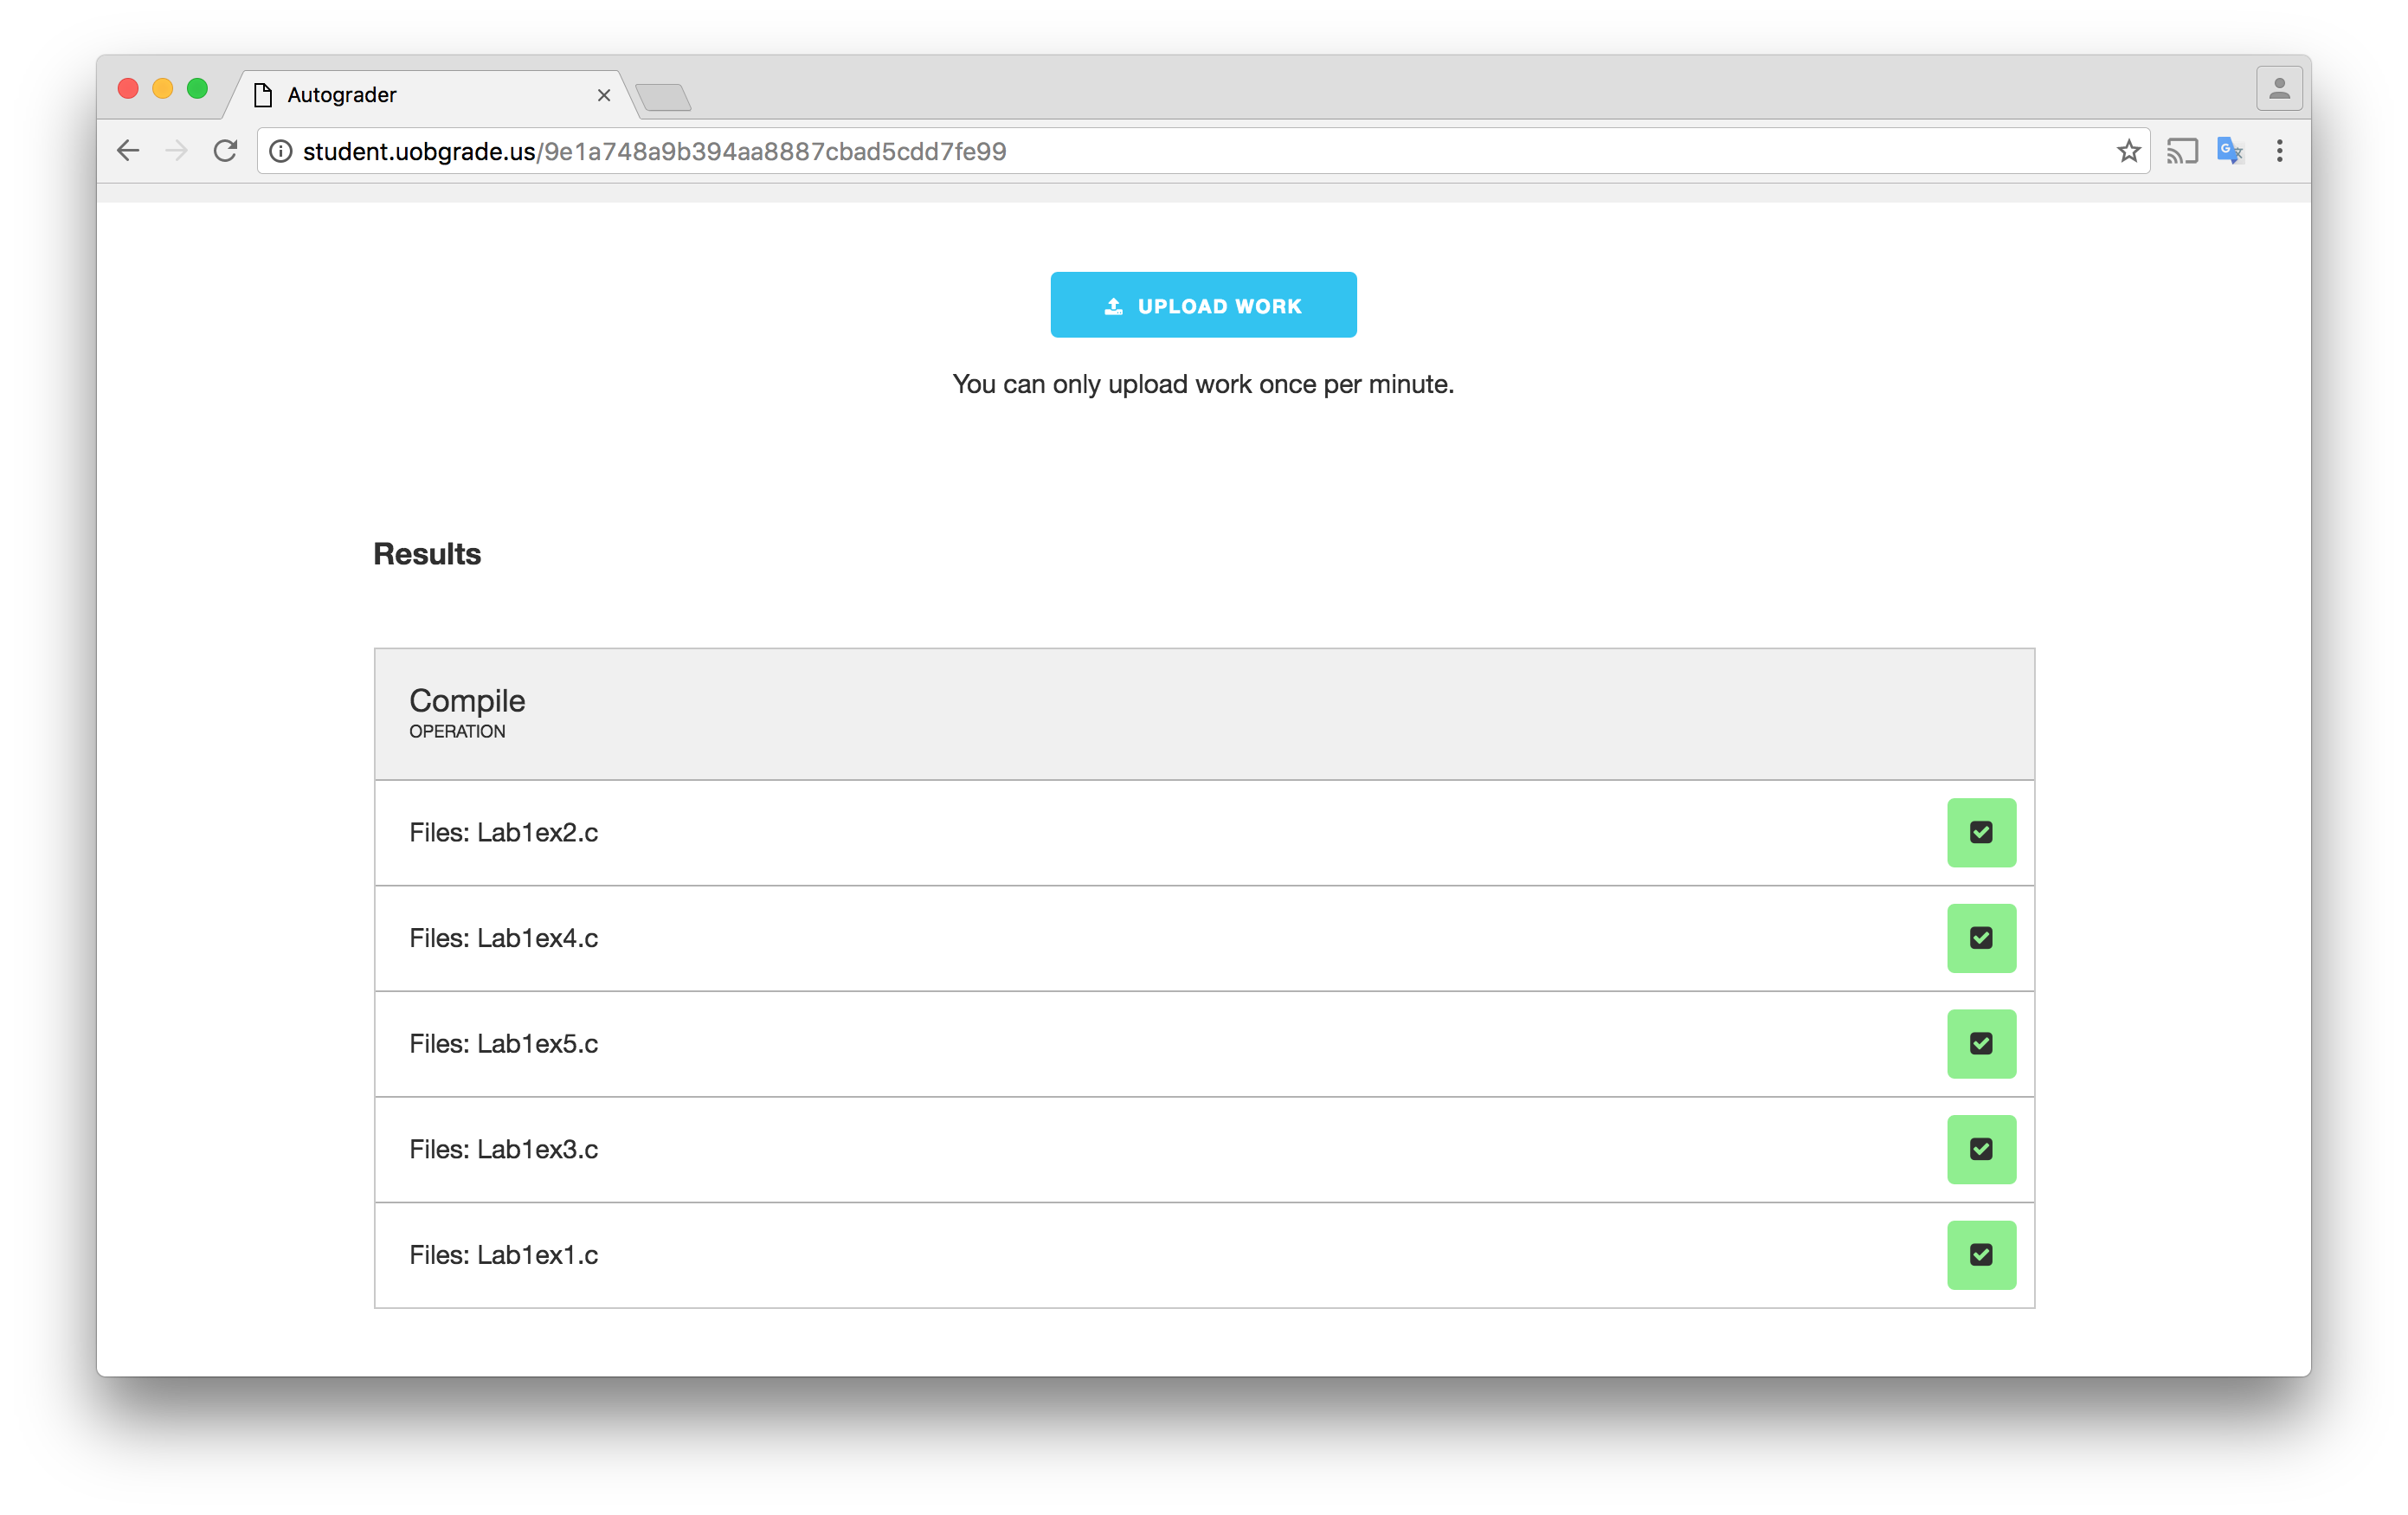
\includegraphics[scale=0.12]{Auto2.png}
\end{frame}

\begin{frame}
Feedback
\begin{itemize}
\item Formative: tutors during \ labs (please ask!)
\item Lab sheets

\begin{itemize}
\item some realtime feedback via the marking tool
\item individual feedback via Moodle
\end{itemize}
\item Larger Courseworks:

\begin{itemize}
\item detailed individual feedback via Moodle
\item general feedback on Moodle
\item tutors and lecturer (please ask!)
\end{itemize}
\item Exam: No individual feedback allowed. Marks will be provided via Moodle.
\end{itemize}
\end{frame} 

\begin{frame}

Exam

\begin{itemize}
\item In the exam, you will be asked to answer 3 questions out of 5 on

\begin{itemize}
\item general programming principles
\item specifics of the C and Java languages
\end{itemize}
\item You may also be asked to 

\begin{itemize}
\item write small programs
\item debug small programs
\item explain the output of small programs
\end{itemize}
\end{itemize}
\end{frame} 

\begin{frame}[fragile]

\begin{lstlisting}
                    Questions? 
\end{lstlisting}
\end{frame} 

\end{document}
